\documentclass[12pt,a4paper,openright,twoside,table]{book}
\usepackage[utf8]{inputenc}
\usepackage{disi-thesis}
\usepackage{code-lstlistings}
\usepackage{listings}
\usepackage{notes}
\usepackage{shortcuts}
\usepackage{acronym}
\usepackage{float}
\usepackage[normalem]{ulem}
\useunder{\uline}{\ul}{}

% Commands
\newcommand\tab[1][1cm]{\hspace*{#1}}

\school{\unibo}
\programme{Corso di Laurea in Ingegneria e Scienze Informatiche}
\title{Monitoraggio Ed Automazione Della Distribuzione Di Software Complessi}
\author{Marco Sternini}
\date{\today}
\subject{Programmazione ad oggetti}
\supervisor{Dott. Danilo Pianini}
\cosupervisor{Dott.sa Martina Baiardi}
\session{III}
\academicyear{2022-2023}

% Definition of acronyms
\acrodef{vm}[VM]{Virtual Machine}
\acrodef{cicd}[CI/CD]{Continuous Integration Continuous Delivery}
\acrodef{cli}[CLI]{Command Line Interface}
\acrodef{jvm}[JVM]{Java Virtual Machine}
\acrodef{jre}[JRE]{Java Runtime Environment}
\acrodef{aur}[AUR]{Arch User Repository}
\acrodef{dsl}[DSL]{Domain-Specific Language}
\acrodef{kiss}[KISS]{Keep It Simple, Stupid}
\acrodef{dry}[DRY]{Don't Repeat Yourself}
\acrodef{jdk}[JDK]{Java Development Kit}
\acrodef{jit}[JIT]{Just in Time}
\acrodef{aot}[AOT]{Ahead of Time}

\mainlinespacing{1.241} % line spacing in mainmatter, comment to default (1)

\begin{document}

\frontmatter\frontispiece

\begin{abstract}	
Max 2000 characters, strict.
\end{abstract}

\begin{dedication} % this is optional
Optional. Max a few lines.
\end{dedication}

\begin{acknowledgements} % this is optional
Optional. Max 1 page.
\end{acknowledgements}

%----------------------------------------------------------------------------------------
\tableofcontents   
\listoffigures     % (optional) comment if empty
\lstlistoflistings % (optional) comment if empty
%----------------------------------------------------------------------------------------

\mainmatter

%!TEX root = ../thesis-main.tex

\chapter{Introduzione}\label{chap:introduction}
Il mondo del software ha scritto diverse decadi di storia. Sin dagli anni '50, quando i primi calcolatori programmabili hanno fatto il loro ingresso sul mercato, il software ha assunto un ruolo sempre più pervasivo nella vita quotidiana delle persone. Oltre ad essere parte integrante dei sistemi informativi delle aziende, lo possiamo trovare anche all'interno di automobili, elettrodomestici e tantissimi strumenti con la quale abbiamo a che fare nella nostra quotidianità. La crescente diffusione del software ha introdotto la necessità di progettare metodologie di sviluppo solide e versatili. Uno dei primi è il \textbf{modello a cascata} il quale struttura il processo di realizzazione del software in fasi sequenziali lineari. Il modello riprende la tipica organizzazione della produzione manifatturiera e fu progressivamente abbandonato con l'evolversi delle richieste del mercato. Successivamente prese piede il concetto di modelli iterativi come il \textbf{modello a spirale} in cui il processo di sviluppo è suddiviso in fasi multiple ripetute più volte (iterazioni). Gli ultimi decenni hanno dato vita a un nuovo modello, considerato lo standard dell'industria, la \textbf{metodologia agile}. Quest'ultima non rappresenta un unico modello, ma un insieme di modelli iterativi costruiti sulla base dei principi definiti all'interno del manifesto agile. Questi principi mettono in primo piano un ambiente autonomo e dinamico in cui sono fondamentali: cicli di sviluppo brevi, continui miglioramenti, la comunicazione col cliente e la consegna tempestiva di funzionalità. Il progetto esposto in questo documento introduce un evoluzione del concetto agile nato recentemente nel mondo dello sviluppo del software, conosciuto come ``DevOps".

\section{Contesto}
Con l'avvento di Internet il concetto di software come un entità sviluppata e finita ha completamente cessato di esistere. Mediante la rete è diventato semplice ed efficiente distribuire un programma e fornire un ulteriore supporto attraverso aggiornamenti evolutivi e correttivi. Il fenomeno è cresciuto tanto da aver dato luce alla pratica del rilascio di applicazioni deliberatamente non complete, le quali attraverso il feedback degli utenti evolvono verso un prodotto finito. Il manifesto agile ha introdotto la cultura di emettere frequenti rilasci di nuove versioni del software, rendendo la distribuzione un punto cardine all'interno del ciclo di vita di esso. Dietro lo sviluppo rapido di nuove funzionalità è necessario il rilascio di queste altrettanto velocemente, la filosofia DevOps nasce per soddisfare questa esigenza.

\subsection{DevOps}
La filosofia DevOps (termine nato dalla contrazione di ``Development" ed ``Operations") si è formata intorno al 2008 con l'idea chiave di unire il team di sviluppo ed il team operativo. Il principale catalizzatore di questo concetto è stata la necessità di affrontare inefficienze nelle fasi del ciclo di vita del software. Differentemente dalla metodologia agile, DevOps è una filosofia di sviluppo software che esprime attraverso tre pilastri il suo obiettivo:

\begin{itemize}
	\item il \textbf{flusso}, il miglioramento del flusso di lavoro lungo l'intero processo di produzione, ciò significa ottimizzare il processo dall'idea, fino alla generazione di valore con il software in produzione.
	\item Il \textbf{feedback}, mediante cicli di feedback rapidi si garantisce la scoperta di difetti nel codice nelle fasi iniziali del ciclo di vita del prodotto. Ciò comporta rapide correzioni, minor debito tecnico e la garanzia di possedere in qualsiasi momento un software stabile e qualitativamente pronto ad un rilascio.
	\item L'\textbf{apprendimento continuo}, la filosofia DevOps promuove la sperimentazione continua, ossia interrogarsi regolarmente sui possibili miglioramenti attuabili assumendosi i rischi che l'applicazione di questi può recare.
\end{itemize}

Le nozioni fornite dalla cultura DevOps ricoprono diversi ambiti e non si limitano agli aspetti tecnici del ciclo di vita del software. Nella pratica esistono diverse tecnologie che concorrono allo sviluppo di processi conformi alla filosofia presentata.

\begin{figure}[htb]
	\centering
	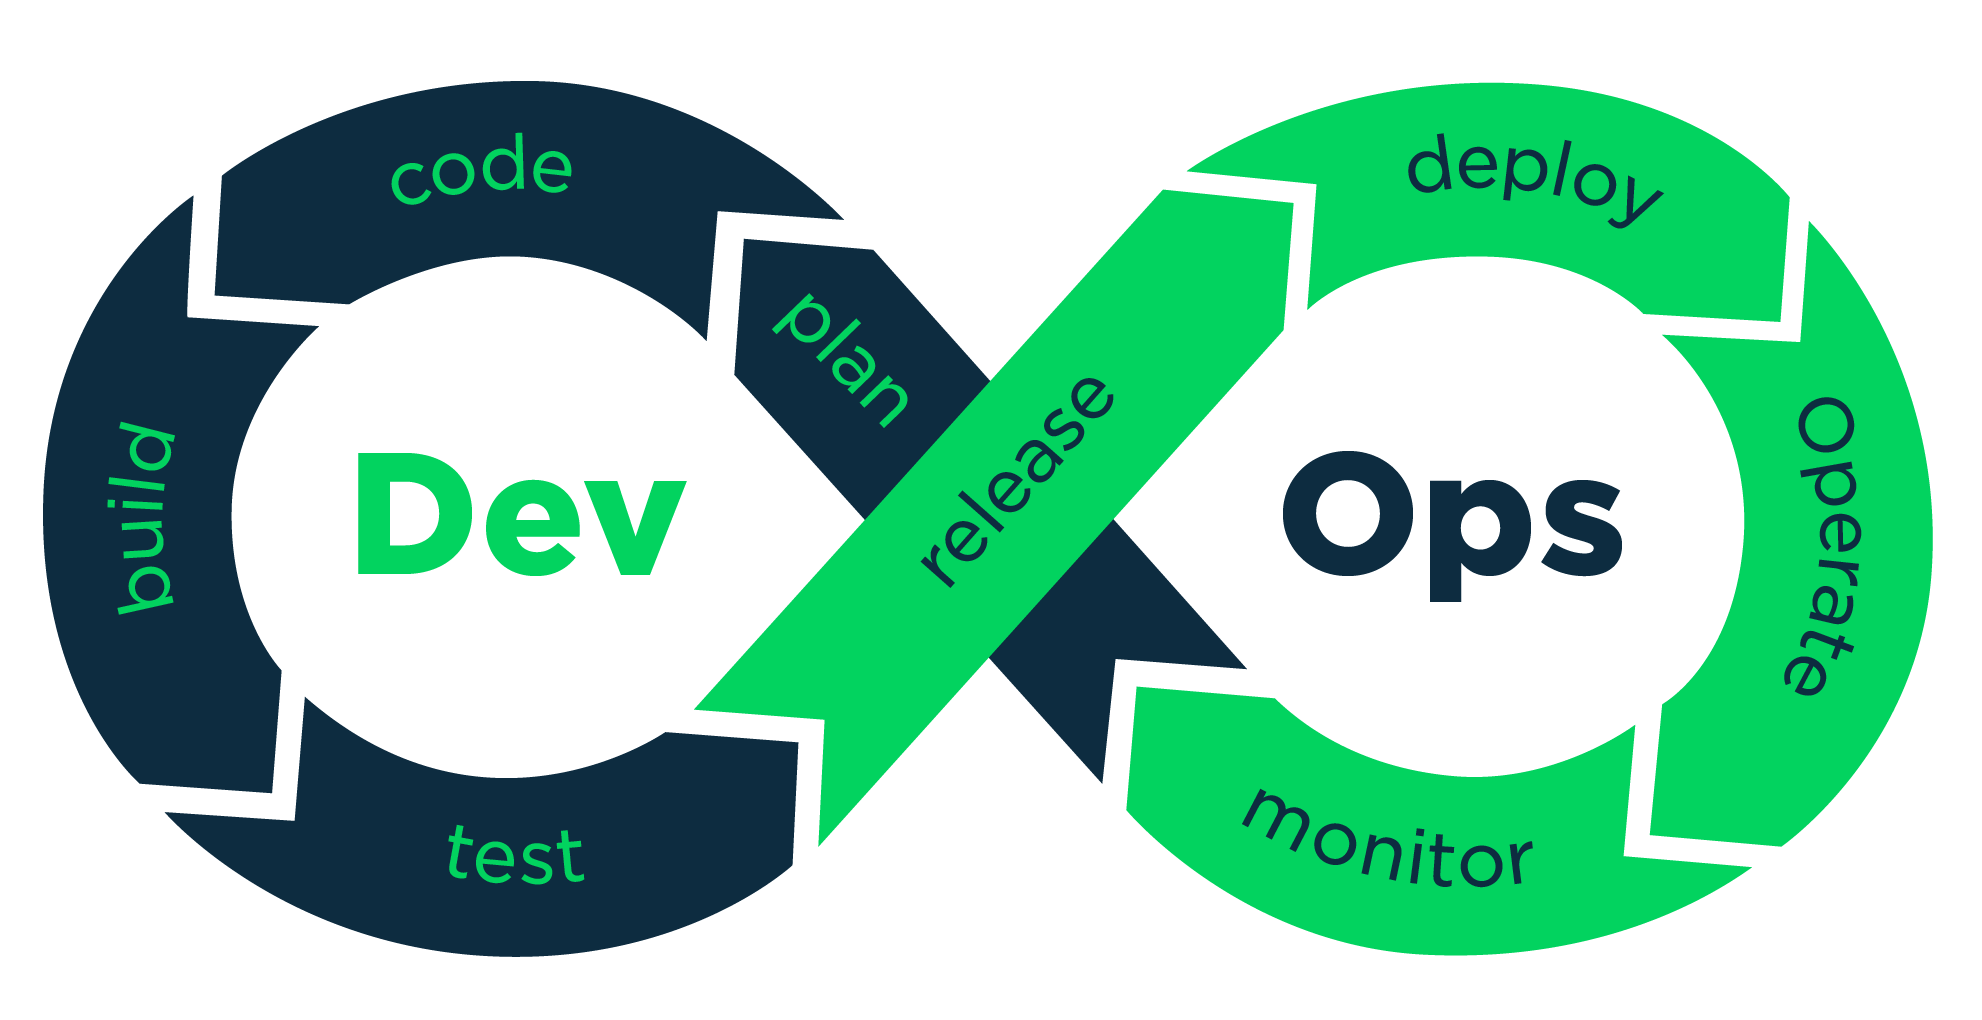
\includegraphics[width=.8\linewidth]{figures/devops-process.png}
	\caption{Le fasi della metodologia DevOps}
	\label{fig:devops-process}
\end{figure}

Il modello illustrato nella figura \ref{fig:devops-process} rappresenta il ciclo di vita del software secondo la filosofia DevOps. La disposizione delle fasi, configurata in modo da evocare il simbolo dell'infinito, simboleggia il concetto di continuità fondamentale per questa filosofia. Questo concetto è introdotto all'interno del flusso mediante un altro pilastro: l'\textit{automazione}. Grazie all'automazione, gli sviluppatori possono delegare compiti complessi o ripetitivi a sistemi esterni configurando tre componenti chiave: un evento, un'azione e il risultato atteso. Quando si verifica un evento specifico, un'entità esterna esegue un insieme di azioni predeterminate, il cui successo o fallimento viene determinato dal confronto con il risultato atteso. A livello pratico, ciò è ottenuto mediante l'utilizzo di server o più generalmente infrastrutture cloud complesse.

L'automazione dunque garantisce l'esecuzione dei processi in modo consistente e permette di concentrare le risorse del team sullo sviluppo, eliminando quindi l'intervento umano da compiti ripetitivi e passibili di errori. Una delle pratiche più diffuse, concetto rilevante della filosofia DevOps, è la pipeline di \ac{cicd}.

\paragraph{Continuous integration} La pratica della \textit{continuous integration} si concentra sull'integrazione automatica e continua delle modifiche al codice sorgente del progetto. Tipicamente, il processo si articola nei seguenti passaggi: (i) gli sviluppatori introducono nuovo codice nel progetto attraverso il software di \textit{version control}, (ii) un server acquisisce le modifiche, compila e testa l'intero progetto, (iii) una volta completato il processo, comunica agli sviluppatori l'esito delle operazioni. Questo approccio consente di individuare errori nel codice anticipatamente, garantendo stabilità e una maggiore qualità al software.

Un aspetto fondamentale è la stesura dei test: un'eccessiva copertura può rallentare il processo di integrazione. È pertanto essenziale bilanciare la copertura dei test in base alle esigenze del progetto, tenendo presente che un aumento della copertura riduce il rischio di introdurre codice difettoso.

\paragraph{Continuous delivery} La distribuzione rappresenta l'insieme di operazioni finalizzate alla consegna del software agli utenti finali. Questo processo estende l'integrazione continua e si preoccupa di garantire la disponibilità costante di un artefatto di build pronto per il rilascio. L'effettivo rilascio di una nuova versione del software può avvenire in modo automatico oppure manualmente da parte dello sviluppatore. La filosofia DevOps fornisce linee guida e non regole rigide, lasciando al team di sviluppo il compito di progettare ed integrare un flusso adeguato alle necessità del progetto.

\subsection{Software JVM-based}
Per "software \ac{jvm}-based" si intendono i programmi e le applicazioni realizzate mediante linguaggi di programmazione eseguiti e compilati per la \ac{jvm}. Nata nel 1995, la Java Virtual Machine ha rivoluzionato il mondo dello sviluppo del software introducendo un nuovo livello di astrazione nella compilazione ed esecuzione dei programmi. Il linguaggio Java, sviluppato appositamente per l'omonima macchina virtuale, è un linguaggio di programmazione ad alto livello orientato agli oggetti progettato per avere il minor numero di dipendenze esterne possibile, in modo da garantire la sua portabilità. L'esecuzione di un programma Java avviene per fasi differenti rispetto ad un normale linguaggio compilato: il codice viene tradotto, in una prima fase di compilazione, in \textit{bytecode}, un linguaggio intermedio. Quest'ultimo è successivamente fornito alla macchina virtuale, la quale interpreta il bytecode generato ed esegue quindi il programma.

Inizialmente progettata per ospitare il linguaggio Java, nel corso del tempo la \ac{jvm} ha visto l'adozione di diversi altri linguaggi di programmazione e l'adattamento di alcuni provenienti da ambienti diversi. Il suo impatto nel mondo del software fu ed è ancora attualmente rilevante, tanto che due indici di valutazione della popolarità dei linguaggi di programmazione posizionano i due principali linguaggi \ac{jvm} all'interno della top 20, con Java, il più datato, nella top 5 (TIOBE\footnote{https://www.tiobe.com/tiobe-index/} e PYPL\footnote{https://pypl.github.io/PYPL.html} index). Una delle caratteristiche che ha decretato il successo di questa architettura è la portabilità. L'integrazione di un linguaggio intermedio permette di astrarre dalla piattaforma di esecuzione, consentendo, mediante un singolo codice sorgente, di distribuire l'applicativo su differenti sistemi operativi con persino architetture hardware diverse.

% Nella figura \ref{fig} è illustrato

Un aspetto cruciale nel rilascio di un'applicazione è la sua distribuzione. La forma e il metodo adottati devono garantire un processo di installazione scorrevole, privo di intoppi e consistente, in modo che gli utenti possano installare l'applicativo nel proprio sistema senza preoccuparsi di dipendenze esterne. Tuttavia, questa necessità presenta sfide specifiche nell'ambito dei linguaggi di programmazione interpretati, come quelli \ac{jvm}-based.

\subsection{Problemi della pacchettizzazione nei software JVM}
L'esecuzione di un programma Java richiede inevitabilmente la presenza di una \ac{jvm}, o più precisamente un \ac{jre}, ossia un ambiente di esecuzione opportuno. Generalmente i software sono distribuiti mediante due tipologie di archivi differenti.

\section{Obiettivi}
I punti discussi precedentemente hanno evidenziato l'importanza che l'automazione ricopre all'interno dello sviluppo del software. Il rilascio continuo di un applicazione è necessario per mantenere elevati standard di qualità e comporta la necessità di automatizzare questi processi per garantire la loro esecuzione in modo consistente. Inoltre, la distribuzione dell'applicativo deve avvenire mediante mezzi compatibili e diffusi per assicurare un processo di installazione semplice e funzionale agli utenti. Il package management system in questo ambito offre un approccio valido: le diverse distribuzioni Linux adoperano esso dagli albori e nei restanti due sistemi operativi, Windows e MacOs, il suo utilizzo si sta diffondendo sempre maggiormente.
\begin{figure}[htb]
	\centering
	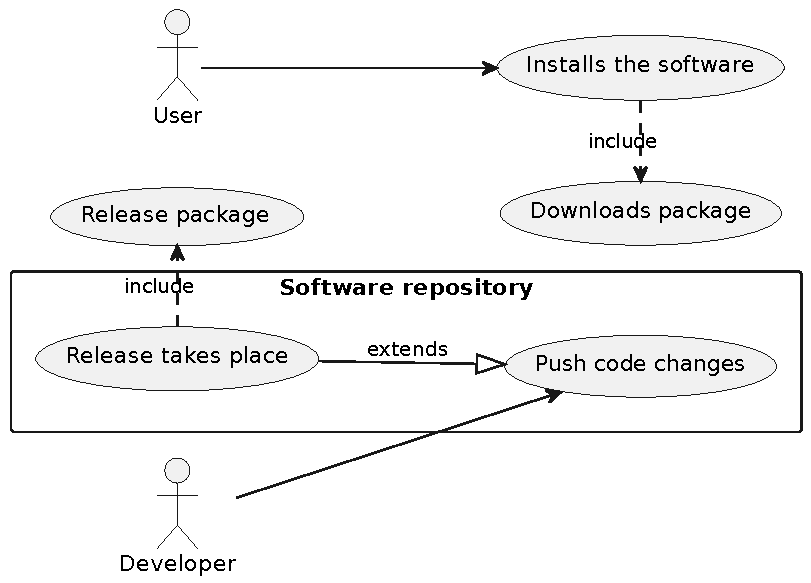
\includegraphics[width=.75\linewidth]{figures/use-case-diagram.pdf}
	\caption{Diagramma dei casi d'uso dallo sviluppatore all'utente}
	\label{fig:use-case-diagram}
\end{figure}

L'obiettivo principale dell'elaborato è quindi quello di progettare un sistema di pacchettizzazione e distribuzione del software automatico all'interno di una pipeline di integrazione e distribuzione continua. I nuovi processi devono integrarsi all'interno dell'attuale pipeline di Alchemist, estendendo le funzionalità di assemblaggio e rilascio del software. La distribuzione del pacchetto software deve avvenire per mezzo di repository pubblici diffusi, in modo da raggiungere il numero maggiore possibile di utenti; essa, inoltre, deve avvenire consistentemente nell'istante in cui una nuova versione di Alchemist viene rilasciata. La totalità dei processi integrati, inoltre, deve prevedere l'esecuzione di test all'interno del flusso, in modo da fornire un riscontro immediato nell'eventualità gli artefatti siano difettosi. Nella \Cref{fig:use-case-diagram} sono rappresentati gli scenari di utilizzo da parte degli utenti finali e degli sviluppatori di Alchemist. In particolare, lo sviluppatore introduce nuovo codice all'interno del repository del progetto e successivamente l'esecuzione della pipeline determina se è necessario il rilascio di una nuova versione. In caso di esito positivo, vengono generati i pacchetti software di installazione. Questi pacchetti, una volta distribuiti, consentiranno agli utenti di introdurre Alchemist nel proprio sistema.
%!TEX root = ../thesis-main.tex
\chapter{Analisi}

\section{Requisiti}

Il progetto si pone due principali obiettivi:
\begin{itemize}
	\item La generazione automatica di pacchetti di installazione multi-piattaforma \\ con \ac{jre} integrato.
	\item La pubblicazione automatica dei rilasci del software all'interno di repository pubblici selezionati.
\end{itemize}
Un pacchetto software è un insieme di risorse necessarie per eseguire un'applicazione o un servizio su un sistema. Sono usualmente distribuiti all'interno di archivi compressi contenenti meta-dati quali: nome, descrizione, versione e dipendenze, pacchetti esterni necessari all'esecuzione. La pubblicazione è l'atto di inserire il software in archivi (repository) online con l'intento di consentire l'installazione agli utenti finali. Entrambi i processi devono essere automatizzati ed integrati all'interno di una pipeline di integrazione e rilascio continua.

\paragraph{Requisiti funzionali}

Le funzionalità richieste si possono classificare in due gruppi distinti: il primo contiene tutto ciò che concerne l'esperienza dell'utente finale, mentre il secondo descrive le funzionalità dal punto di vista degli sviluppatori e contributori di Alchemist. Di seguito il primo gruppo:
\begin{itemize}
	\item \textbf{Pacchettizzazione}: il simulatore deve essere distribuito in pacchetti auto-contenuti, ossia comprendenti di tutto il necessario per l'utilizzo di esso.
	\item \textbf{Multi-piattaforma}: Alchemist deve essere installabile sui maggiori sistemi operativi in circolazione come Windows, MacOS e le principali distribuzioni Linux.
	\item \textbf{Plug and play}: l'installazione non deve richiedere configurazioni complesse, l'applicativo deve essere pronto all'uso non appena installato.
\end{itemize}

I requisiti del gruppo successivo sono accumunabili per il loro scopo, vale a dire l'automazione.

\begin{itemize}
	\item \textbf{Automazione dei pacchetti}: la generazione dei pacchetti di installazione deve essere automatica e configurabile
	\item \textbf{Automazione della distribuzione}: il rilascio di una nuova versione comprende la distribuzione di essa nei repository selezionati e deve essere svolta in modo automatico.
	\item \textbf{Verifica funzionamento}: entrambi i processi descritti precedentemente devono essere corredati da verifiche del loro funzionamento e devono bloccare la procedura di rilascio nell'eventualità siano presenti errori.
\end{itemize}

\paragraph{Requisiti non funzionali}

\begin{itemize}
	\item Trattandosi Alchemist di un software in continuo sviluppo, è auspicabile l'utilizzo degli strumenti già impiegati all'interno del repository. \\ L'integrazione di nuovi applicativi deve essere eseguita solo se strettamente necessaria.
	\item La pipeline \ac{cicd} ottenuta deve garantire prestazioni in linea con la versione precedente l'intervento di questo progetto.
\end{itemize}

\section{Pacchettizzazione}\label{sec:packaging}

Come si evince dall'analisi svolta, la pacchettizzazione è requisito fondamentale dell'elaborato. Sino ad ora l'applicativo Alchemist era distribuito in file JAR, ossia archivi java compressi contenenti tutte le dipendenze ed i relativi \textit{classfiles} necessari all'esecuzione. Quest'approccio molto diffuso porta con sè diverse limitazioni tra cui:
\begin{itemize}
	\item la necessità dell'utente scaricante di avere un \ac{jre} installato nel proprio dispositivo,
	\item il potenziale bisogno di utilizzare un ambiente \ac{jre} specifico e quindi per l'utente di non possedere una versione dell'ambiente compatibile,
	\item la difficoltà di utilizzo per utenti non esperti, i quali sono abituati ad eseguire programmi utilizzando file eseguibili nativi della propria piattaforma.
\end{itemize}

Seppur alcune di queste restrizioni sono in parte mitigate in certe piattaforme, non è lo stesso per altre molto diffuse come Windows, il quale per esempio non fornisce un ambiente java pre-installato. Esistono diversi strumenti di terze parti e non che cercano di far fronte a questo problema, è importante dunque valutare e scegliere lo strumento più opportuno.

\subsection{Soluzioni}

Nell'ottica di semplificare la configurazione di questo processo lo strumento selezionato deve supportare le tre principali piattaforme descritte nei requisiti precedentemente. Tra gli strumenti analizzati due molto differenti si sono distinti, vale a dire: \textit{jpackage}, comando disponibile nel \ac{jdk} dalla versione 14 adibito alla produzione di pacchetti auto-contenuti con \ac{jre} integrata e \textit{GraalVM}, un \ac{jdk} sviluppato da Oracle che fornisce un compilatore \ac{jit} e \ac{aot} per java. Il termine \ac{jit} descrive il comportamento normale di ogni \ac{jvm}: il \textit{java compiler} traduce il programma ad alto livello in \textit{bytecode}, successivamente la \ac{jvm} trasforma il bytecode in linguaggio macchina specifico per l'architettura sottostante eseguendo dunque una compilazione dinamica. In contrasto la tecnica \ac{aot} ricorda i linguaggi di programmazione compilati, la compilazione è statica ed avviene prima dell'esecuzione del programma. Il compilatore \ac{aot} chiamato ``Native Image", consente di compilare un programma java (ed altri linguaggi di programmazione) ottenendo in output un eseguibile nativo per ogni piattaforma. Quest'ultimo inoltre porta con sè diversi vantaggi come: un minor costo in risorse CPU e memoria, tempi di avvio minori e dimensioni ridotte rispetto un normale programma java distribuito con un \ac{jre}. L'annessione di un JRE è superfluo, l'eseguibile prodotto contiene tutto il necessario per l'esecuzione dell'applicazione. La compilazione \ac{aot} però ha dei requisiti, uno di questi fondamentale è la \textit{closed world assumption}: ossia ogni parte di codice raggiungibile in esecuzione lo deve essere anche in fase di build, altrimenti l'eseguibile finale sarà incompleto. Ciò accade perché native image svolge un analisi statica del codice, alcune funzionalità come la reflection oppure il caricamento dinamico non sono supportate e richiedono una soluzione alternativa.

In contrasto jpackage fornisce uno strumento interessante, il quale non richiede modifiche all'applicativo ed è pre-installato in tutti i \ac{jdk} dalla versione 14 e successive. Supporta nativamente l'annessione di un \ac{jre} utilizzando \textit{jlink}, produce diverse tipologie di pacchetti per ogni piattaforma ed è completamente controllabile da interfaccia \ac{cli}. Le tipologie di pacchetti generabili sono elencate di seguito:
\begin{itemize}
	\item EXE e MSI per Windows
	\item RPM e DEB per Linux
	\item PKG e DMG per MacOs.
\end{itemize}
Anch'esso presenta dei limiti come: la necessità di essere eseguito sullo stesso sistema operativo dove i pacchetti prodotti sono destinati (lo stesso vale per GraalVM, la \textit{cross compilation} non è supportata) e la produzione di un solo pacchetto ad ogni esecuzione.

\paragraph{Valutazione finale} Ambedue le soluzioni concorrono all'obiettivo primario, la distribuzione del software multi-piattaforma e pronto all'uso. GraalVM fornisce diversi vantaggi prestazionali, ma i requisiti da esso richiesti non sono compatibili con l'architettura del simulatore. D'altro canto jpackage fornisce tutto il necessario per costruire i pacchetti con embed di un \ac{jre} e i limiti delineati sono superabili adoperando script o configurazioni specifiche.

\section{Strumenti}

\subsection{Gradle}

Mentre in passato la produzione di artefatti (documentazione, pacchetti, eseguibili) era delegata a script costruiti dallo sviluppatore, in un progetto di grandi dimensioni è oggigiorno essenziale avvalersi di uno strumento di build automation. Come l'output di un programma deterministico non cambia per uno stesso input, la produzione di artefatti deve essere consistente e riproducibile riducendo al minimo l'intervento umano. 

Gradle è uno dei tanti strumenti disponibili, supporta diversi linguaggi di programmazione anche se risulta popolare nell'ambiente JVM come alternativa a Maven. I \textit{task} sono l'unità minima di esecuzione e rappresentano un azione: come generare un JAR, eseguire dei test o produrre la documentazione. Mediante direttive come \textit{dependsOn} è possibile creare dipendenze tra processi, Gradle per orchestrare l'esecuzione dei task costruisce un grafo aciclico diretto (DAG) delle dipendenze. L'esecuzione di Gradle avviene in tre fasi distinte elencate di seguito.
\begin{enumerate}
	\item \textbf{Fase di inizializzazione}. In primo luogo Gradle crea un'istanza di Settings che organizza l'architettura del progetto. Attraverso un file, di nome ``settings.gradle", lo sviluppatore stabilisce il progetto radice e tutti gli eventuali progetti figli. 
	\item \textbf{Fase di configurazione}. Successivamente tutti i file di configurazione ``build.gradle" (del progetto radice e tutti i sotto-progetti) vengono analizzati per costruire il grafo dei task.
	\item \textbf{Fase di esecuzione}. Infine, Gradle esegue i task richiesti considerando le dipendenze descritte nel grafo generato nella fase precedente.
\end{enumerate}

\begin{figure}[htb]
	\centering
	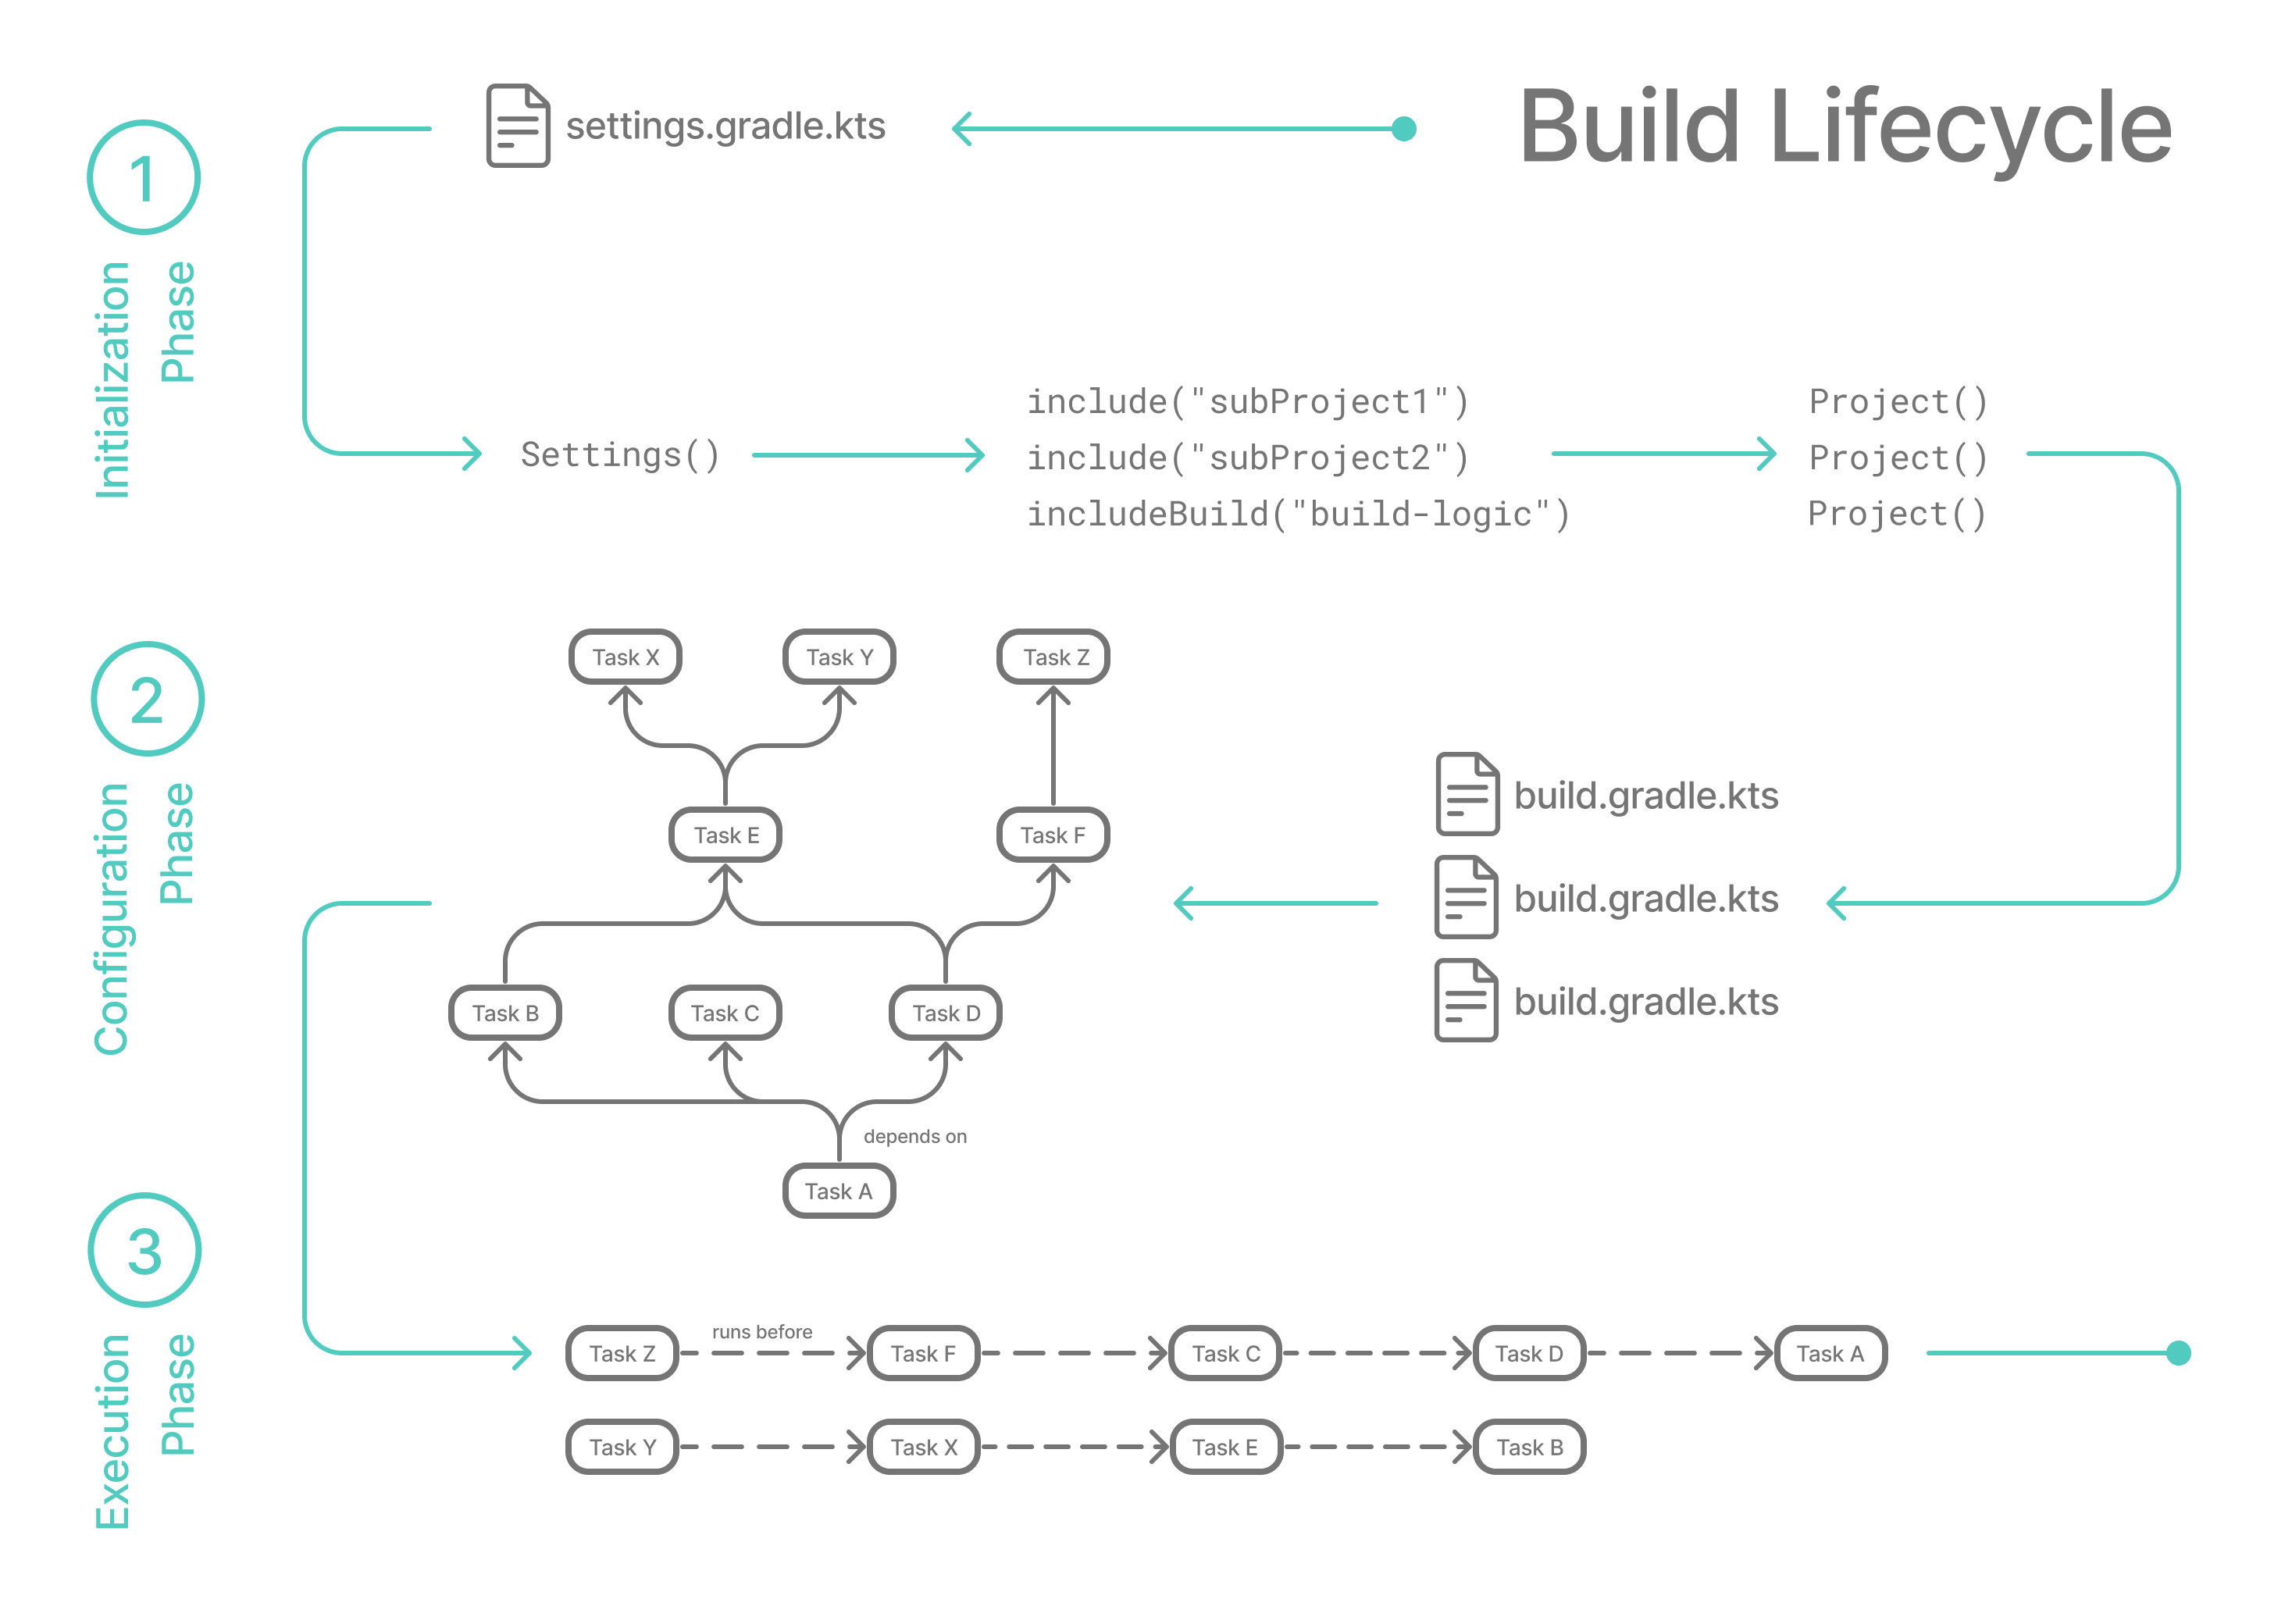
\includegraphics[width=.9\linewidth]{figures/gradle-build-lifecycle-example.png}
	\caption{Esempio di inizializzazione, configurazione ed esecuzione di una build Gradle}
	\label{fig:gradle-build-lifecycle}
\end{figure}

Un componente chiave sono i plugin, i quali consentono di estendere le funzionalità di Gradle: aggiungere nuovi task, estendere il modello con nuovi elementi ed applicare configurazioni specifiche all'intero progetto. La presenza di diversi plugin base e creati dalla comunità rende Gradle uno strumento versatile.

\paragraph{Analisi rispetto ai requisiti}
In considerazione dei requisiti di automazione, Gradle fornisce le funzionalità necessarie a soddisfare i requisiti di pacchettizzazione, distribuzione e verifica del funzionamento. Utilizzando Gradle si integrano questi processi all'interno del build system garantendo un corretto ordine di esecuzione con l'effetto di minimizzare l'incidenza di errori e assicurando la produzione di pacchetti conformi su qualsiasi sistema operativo questo venga eseguito.
L'approccio orientato ai task inoltre permette di suddividere un macro-processo in più unità di esecuzione riutilizzabili da altri processi, garantendo tutti i vantaggi che la filosofia \ac{dry} fornisce.

\subsection{GitHub Actions}

Tramite Gradle lo sviluppatore è in grado di eseguire procedure articolate come compilazione, test e dispiegamento utilizzando un semplice comando da \ac{cli}. L'e\-se\-cu\-zio\-ne di queste procedure richiede però l'intervento umano, è quindi necessario uno strumento capace di automatizzare queste procedure offrendo un infrastruttura resiliente e facilmente accessibile.

GitHub Actions è una piattaforma per automatizzare processi di \ac{cicd} disponibile per i repository ospitati su GitHub. Gli sviluppatori utilizzano esso per eseguire automaticamente test ad ogni commit, controllare il codice fornito dai contributori o distribuire regolarmente l'applicazione. Consente la configurazione ed esecuzione di pipeline personalizzate, ovvero i \textit{workflow} processi eseguibili consistenti in un insieme di \textit{job} eseguiti sequenzialmente o parallelamente all'interno di macchine virtuali dette \textit{runner}. I workflow vengono eseguiti quando un certo evento, configurato dallo sviluppatore, si manifesta. GitHub in primo luogo è una piattaforma di code-sharing orientata allo sviluppo open source, una peculiarità della funzionalità Actions è la vasta gamma di eventi legati alla piattaforma: dall'apertura di una pull-request, un commento o la creazione di un fork.

I workflow (figura \ref{fig:github-actions-example}) sono descritti in file YAML all'interno di una cartella specifica del repository. In primis si configura il nome del workflow e l'evento che origina l'esecuzione di esso, successivamente l'elenco dei job e gli step, l'unità di esecuzione minima che raggruppate modellano l'azione svolta dal job.

\begin{figure}[htb]
	\centering
	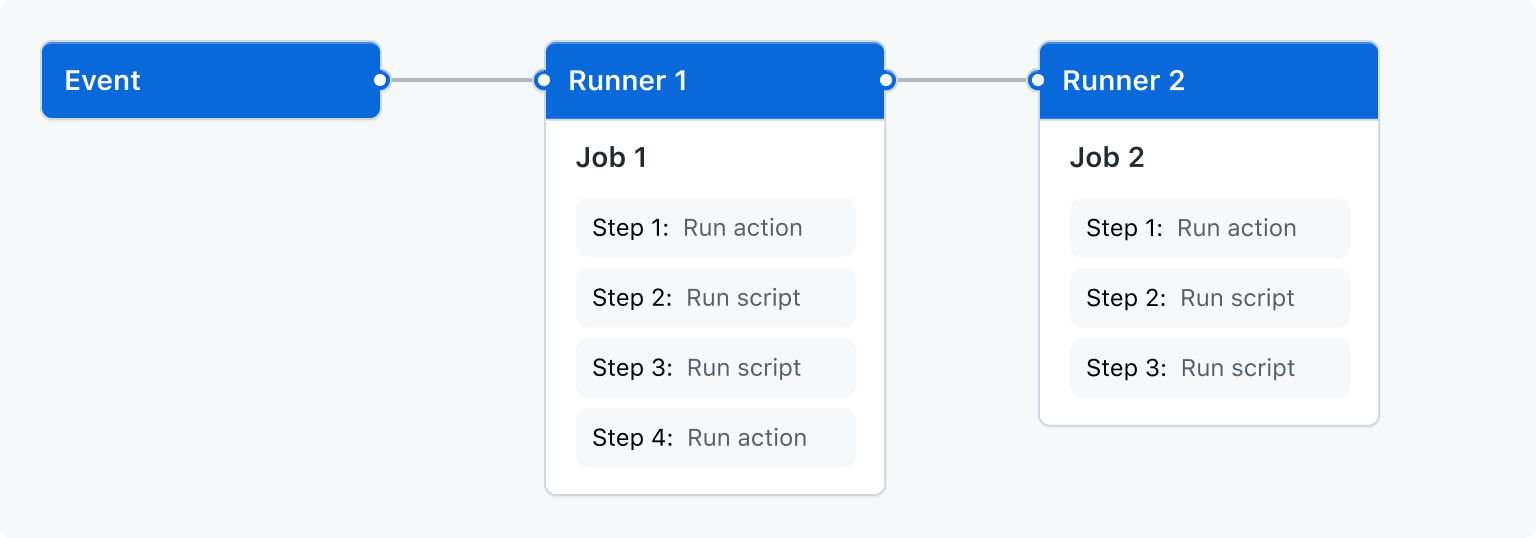
\includegraphics[width=.9\linewidth]{figures/overview-actions-simple.png}
	\caption{Sintesi dei componenti utilizzati su GitHub Actions ed esempio di un workflow \\ source: https://docs.github.com/en/actions/learn-github-actions/understanding-github-actions}
	\label{fig:github-actions-example}
\end{figure}

Uno step può presentare una lista di comandi eseguiti nella shell di riferimento (quella di default per il sistema operativo o un'altra se specificata) altrimenti un'\textit{action}. Le action sono componenti riutilizzabili che eseguono un'attività precisa, esistono diverse azioni sviluppate dalla comunità e rese disponibili all'interno di un marketplace vasto. Per esempio una delle più diffuse ed utilizzate è ``actions/checkout" [\cite{github-actions-diffusion}], la quale clona il repository del progetto nella cartella di lavoro corrente del runner.

\paragraph{Analisi rispetto ai requisiti}

La piattaforma di GitHub Actions ricopre un ruolo fondamentale: offre l'infrastruttura per l'e\-se\-cu\-zio\-ne dei processi quali vogliamo automatizzare. Rispetto ai requisiti risponde con successo presentando:
\begin{itemize}
	\item la possibilità di utilizzare macchine virtuali (runner) di tutte e tre i sistemi operativi target,
	\item la possibilità di configurare eventi o esecuzioni ricorrenti del processo costruito, assicurando quindi l'automazione di quest'ultimo.
\end{itemize}
Riguardo invece i requisti non funzionali, il workflow deve sfruttare le funzionalità di Actions per ottimizzare l'esecuzione del flusso, riducendo i tempi di sviluppo e i costi collegati all'utilizzo della piattaforma.

\subsection{Package manager}

Nei sistemi operativi Linux il controllo dei componenti installati nella macchina è completamente delegato ai \textit{package manager}. Il \textit{package-management system} è un insieme di strumenti software che gestiscono i processi di installazione, aggiornamento, configurazione e rimozione di applicativi dal sistema. Spesso un pacchetto corrisponde ad un particolare programma o applicazione, contemporaneamente però esistono applicativi più complessi composti da numerosi pacchetti correlati. Il sistema di gestione dei pacchetti opera attraverso tre componenti principali.

\begin{itemize}
	\item Un componente a basso livello che si occupa principalmente dell'installazione o rimozione dei pacchetti. Definito come il back-end dei package-management system, è il caso di \textbf{rpm} il quale gestisce gli omonimi pacchetti e dpkg per i pacchetti \textbf{deb}.
	\item Un componente ad alto livello il cui compito principale è quello di fornire un'interfaccia all'utente come: \textbf{yum} per Fedora o \textbf{apt} per Debian. Si occupa inoltre di risolvere le dipendenze e gestire le sorgenti esterne (repository).
	\item I repository, ossia database pubblici ufficiali o no contenenti i pacchetti ed i relativi meta-dati.
\end{itemize}

\begin{figure}[H]
	\centering
	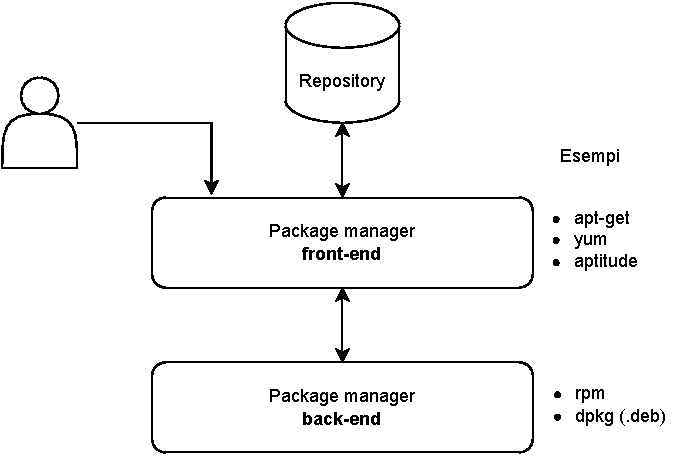
\includegraphics[width=.7\linewidth]{figures/package-managers.pdf}
	\caption{Struttura più diffusa dei sistemi di gestione di pacchetti}
	\label{fig:package-managers}
\end{figure}

\paragraph{Arch User Repository} Una distribuzione importante nel vasto panorama dei fork Linux è Arch. Arch è una distribuzione Linux con architettura x86-64 creata seguendo la filosofia \ac{kiss}. È infatti rinomata per essere leggera, veloce, estremamente scalabile ed adattabile alle proprie esigenze. Data la sua natura minimalista, l'installazione iniziale non incorpora alcun strumento di configurazione automatica, nessun ambiente desktop e nessun altro strumento necessario all'avvio del sistema. Il sistema di gestione dei pacchetti si chiama \textit{pacman} ed a differenza dei concorrenti, opera sia a basso che ad alto livello. Un pacchetto non è altro che un file shell script denominato \textit{PKGBUILD} contenente le istruzioni necessarie a scaricare i sorgenti e compilarli attraverso un comando: \textit{makepkg}. La linearità dei file PKGBUILD rende la creazione di pacchetti alla portata di qualsiasi utente difatti Arch supporta \textbf{\ac{aur}}, un tratto distintivo di questa distribuzione. Si tratta di un repository di pacchetti in cui qualsiasi utente, anche non sviluppatore, può contribuire.  

\paragraph{Windows e winget} Discorso differente vale per Windows, ove fino a poco tempo fa non era previsto alcun package manager ufficiale pre-installato. Gli utenti usualmente installano software attraverso pacchetti distribuiti in siti web ad-hoc, store non ufficiali o attraverso il Microsoft Store, gli sviluppatori invece, per sfruttare tutti i benefici della gestione a pacchetti utilizzano package-management system di terze parti. Solamente nel settembre 2020 è nato ``winget": package-management system open-source sviluppato da Microsoft, il quale supporta pacchetti di installazione EXE, MSIX e MSI. Il repository dei pacchetti è accessibile pubblicamente ed è possibile mediante richieste di contribuzione e previa approvazione, pubblicare pacchetti all'interno di esso.

\paragraph{Pacchetti containerizzati} Un'altra tipologia sono i pacchetti detti containerizzati, ovvero eseguiti all'interno di ambienti separati con un accesso limitato al sistema. Questa caratteristica fornisce due principali vantaggi: la possibilità per una applicazione di usare la propria versione desiderata di librerie di sistema senza creare conflitti e la trasparenza all'utente nell'accesso alle risorse di sistema, garantendo un livello aggiuntivo di sicurezza. È il caso dei pacchetti \textit{snap}, pacchetti auto-contenuti considerati universali perché compatibili con una notevole quantità di distribuzioni Linux. Quest'ultimi sono disponibili ed installabili all'interno dello ``SnapStore", l'unico repository compatibile ed ufficiale.

\paragraph{Analisi rispetto ai requisiti}
Nell'ottica di soddisfare il requisito multi-piat\-ta\-for\-ma del progetto è necessario analizzare le piattaforme di destinazione elencate. Data la natura closed-source di Windows e MacOs, i due sistemi operativi non richiedono particolari attenzioni dato che le tipologie di pacchetti generabili da jpackage sono sufficienti ed ufficialmente supportati. Linux al contrario è notevolmente frammentato, ogni distribuzione è libera di utilizzare il package management system preferito o di inventare una tipologia di pacchetto completamente nuova. Purtroppo non esistono statistiche ufficiali riguardo la diffusione delle distribuzioni, molte di esse si basano su stime o utilizzano dati non attendibili. Dall'altro lato analizzando i pacchetti generabili da jpackage possiamo trarre delle conclusioni.
\begin{itemize}
	\item RPM significa ``RedHat Package Manager", progettato per RedHat e le distribuzioni derivate, risulta diffuso inoltre su Fedora, CentOs, OpenSUSE e tante altre distribuzioni. 
	\item DEB è l'abbreviazione di ``Debian packages", supportato da Debian e le distribuzioni derivate. Secondo distrowatch.com Debian Linux presenta più di 400 distribuzioni derivate e più di 120 di queste sono attive.
\end{itemize}
È evidente come le due tipologie coprono un ampio spettro nel panorama Linux. Queste due tipologie sono inoltre supportate nativamente da PKGBUILD, il quale autonomamente estrae il loro contenuto lasciando allo sviluppatore solamente il compito di riposizionare esso nel filesystem del sistema installante. Il supporto ai pacchetti snap fornisce un ulteriore livello di compatibilità essendo di fatto considerato una tipologia universale nel mondo Linux.

\chapter{Design}

\section{Architettura e macrostruttura}

Alchemist, come esplicato nella sezione 1.4, è un progetto modulare complesso in continuo sviluppo. Gli strumenti presentati nel capitolo precedente trovano già impiego nel progetto, ad eccezione del software di impacchettamento il quale è oggetto di questo elaborato. Di seguito il confronto macro-strutturale riguarda l'utilizzo dell'infrastruttura GitHub Actions.
\paragraph{Architettura iniziale} Alchemist utilizza fondamentalmente due workflow per soddisfare i requisiti di integrazione e rilascio continuo. Un primo workflow chiamato ``dispatcher", il quale funziona come punto di inizio del flusso, è in ascolto di diversi eventi e una volta avviato esamina (inspect) i meta-dati dell'evento scatenante per determinare lo step successivo. In particolare nella configurazione in oggetto questo step iniziale funge da filtro dal momento che esiste un solo possibile step successivo, ossia il secondo workflow quello adibito a soddisfare i compiti di build, test e distribuzione.

\paragraph{}
\section{Flusso di rilascio}
Uno dei requisiti del metodo di sviluppo \ac{cicd} è 


\section{User experience}
Discussione design della terza parte

\subsection{CLI e GUI}

\subsection{Design CLI}

%!TEX root = ../thesis-main.tex

% Percorso implementativo:
% 	V- jpackage e le opzioni in dettaglio
%  	V- jlink e jdeps
%   V- il plugin gradle per operare con jpackage
%   V- la necessità di estendere con jpackageFull
%   - inserimento dei test e della release dei pacchetti
%   - le operazioni per la distribuzione e il test di queste (AUR)

\chapter{Implementazione}

Nel seguente capitolo è illustrato il percorso e le relative scelte implementative effettuate per soddisfare i requisiti posti dal progetto. Successivamente, valuterò il lavoro svolto considerando i requisiti non funzionali posti.

\section{Pacchettizzazione e distribuzione}

\subsection{Pacchettizzazione}
Come discusso nelle precedenti sezioni riguardanti lo strumento jpackage (in particolare sezione \ref{sec:design-jpackage}), esso presenta una notevole quantità di opzioni sia inerenti l'aspetto estetico (come nome dell'applicazione, icona, copyright ed altri), sia riguardo aspetti tecnici che possono contraddistinguere la qualità del pacchetto di installazione.
\def\arraystretch{1.5}
\begin{table}[htb]
	\label{fig:jpackage-options}
	\begin{tabular}{|l|l|l|}
		\hline
		\rowcolor[HTML]{ECF4FF} 
		\multicolumn{1}{|c|}{\cellcolor[HTML]{ECF4FF}{\ul Opzione}} &
		\multicolumn{1}{|c|}{\cellcolor[HTML]{ECF4FF}{\ul Funzionalità}} &
		\multicolumn{1}{|c|}{\cellcolor[HTML]{ECF4FF}{\ul Eventuali parametri}} \\ \hline
		\texttt{--type} &
		Tipologia di pacchetto in output &
		\begin{tabular}[c]{@{}l@{}}rpm, deb, exe, msi, \\ pkg, dmg\end{tabular} \\ \hline
		\texttt{--input} &
		\begin{tabular}[c]{@{}l@{}}Directory contenente i file\\ da impacchettare\end{tabular} &
		Percorso alla directory \\ \hline
		\texttt{--main-jar} &
		\begin{tabular}[c]{@{}l@{}}L'archivio JAR principale\\ contenete la classe principale\end{tabular} &
		Percorso del JAR \\ \hline
		\texttt{--main-class} &
		\begin{tabular}[c]{@{}l@{}}La classe che contiene la \\ funzione di avvio\end{tabular} &
		Nome della classe \\ \hline
		\texttt{--add-modules} &
		\begin{tabular}[c]{@{}l@{}}I moduli integrati nel\\ runtime-image generato da \\ jlink\end{tabular} &
		\begin{tabular}[c]{@{}l@{}}Lista dei moduli separata\\ da ','\end{tabular} \\ \hline
		\texttt{--jlink-options} &
		\begin{tabular}[c]{@{}l@{}}Ulteriori opzioni per\\ l'esecuzione di jlink\end{tabular} &
		Lista delle opzioni \\ 
	\end{tabular}
	\caption{Tabella che elenca le principali opzioni tecniche del comando \texttt{jpackage}}
\end{table}

\paragraph{Ottimizzazione} Per comprendere le scelte implementative riguardo le opzioni di carattere tecnico è necessario introdurre altri due strumenti del \ac{jdk}: (i) \texttt{jlink}, strumento delegato alla produzione della \textit{runtime-image} inserita all'interno del pacchetto e (ii) \texttt{jdeps}, comando utilizzabile per analizzare le dipendenze di un archivio JAR. Il primo ha la peculiarità di consentire la creazione di immagini personalizzate contenente solo i componenti necessari per eseguire un'applicazione specifica, riducendo così le dimensioni complessive e incrementando le prestazioni dell'applicazione. Per ottenere i componenti necessari si utilizza il secondo, jdeps, applicandolo all'archivio JAR contenente l'intera applicazione. In sintesi la generazione del pacchetto richiede l'utilizzo dei tre strumenti consecutivamente come esposto di seguito:
\begin{enumerate}
	\item \texttt{jdeps}, analizza l'archivio contenente la nostra applicazione e restituisce i moduli jvm necessari per il corretto funzionamento di essa.
	\item \texttt{jlink}, utilizza i moduli evidenziati da jdeps per creare una runtime-image personalizzata di dimensioni ridotte
	\item \texttt{jpackage}, utilizza la runtime-image creata precedentemente assieme all'ar\-chi\-vio dell'applicazione per generare il pacchetto: l'application-image.
\end{enumerate}

\lstinputlisting[float,language=Bash,label={lst:jlink-runtime-image-creation}, caption={Comandi eseguiti per creare un java-runtime di dimensioni ridotte}]{listings/jpackage-jlink.sh}

I comandi utilizzati nel processo sono indicati nel listato \ref{lst:jlink-runtime-image-creation}. In particolare l'esecuzione di jdeps coinvolge le seguenti opzioni:
\begin{itemize}
	\item \texttt{--print-module-deps} indica di restituire un output conforme all'input ri\-chie\-sto da jlink,
	\item \texttt{--add-modules} aggiunge attraverso la costante ``ALL-MODULE-PATH" tutti i moduli per eseguire l'analisi,
	\item \texttt{--ignore-missing-deps} non restituisce le dipendenze mancanti nell'output,
	\item \texttt{--no-recursive} esegue un analisi solo al primo livello di dipendenza.
\end{itemize}

Le opzioni configurate nell'utilizzo di jlink sono quelle di default che jpackage utilizza: \texttt{--no-header-files} e \texttt{--no-man-pages} precludono l'inserimento dei file header e dei manuali per diminuire ulteriormente la dimensione della runtime-image.
Il comando jpackage completo utilizzando le opzioni descritte nella tabella \ref{fig:jpackage-options} è il seguente:

\texttt{\\ jpackage --input build/package-input \\ \tab\tab --main-jar alchemist-full-VERSION.jar \\ \tab\tab --main-class it.unibo.alchemist.Alchemist \\ \tab\tab --type \{rpm, deb\} \\ \tab\tab --add-modules \$DEPENDENCIES \\ \tab\tab --jlink-options no-header-file, no-man-pages \\}

%Confronto, scelta tra i due full o solo moduli, il guadagno in %, perché in alchemist è così poco ed in altre applicazioni potrebbe essere molto maggiore, analisi della reflection step necessario al funzionamento

Il risultato ottenuto è interessante, la differenza tra i due dati è buona.
Il simulatore Alchemist è estendibile, ed ottiene questa caratteristica sfruttando la reflection.


%------------------------------------------------

\paragraph{Plugin} Il design elaborato nel capitolo precedente evidenziava la necessità di un task \textit{wrapper} che incapsulasse le opzioni e funzionalità di jpackage. La versatilità offerta da Gradle ha permesso di ottenere il risultato voluto attraverso \textit{jpackage-gradle-plugin}\footnote{https://github.com/petr-panteleyev/jpackage-gradle-plugin}: un plugin sviluppato dalla comunità. Questo componente introduce un tipo di task \texttt{JPackageTask} capace di: (i) configurare tutte le opzioni supportate da jpackage per qualsiasi versione del \ac{jdk}, (ii) definire blocchi eseguiti solamente su un sistema operativo specifico e (iii) testare le configurazioni attraverso la modalità \textit{dry run}. Il plugin introdotto però, non compensa uno dei limiti di jpackage esposto durante l'analisi dello strumento, ossia la necessità di eseguire il programma molteplici volte per ottenere tutte le tipologie di pacchetti. Per far fronte a questa restrizione, ho creato una tipologia personalizzata (listato \ref{lst:custom-jpackage-task}) estendendo quella fornita dal plugin per modificare il suo comportamento in esecuzione, nello specifico il metodo contrassegnato come \texttt{@TaskAction}.

\lstinputlisting[float,language=Kotlin,label={lst:custom-jpackage-task}, caption={Definizione di un tipo personalizzato per compensare il limite di jpackage}]{listings/custom-jpackage-task.kt}

\subsection{Distribuzione}

Una volta impacchettato l'applicativo, quest'ultimo è pronto per essere installato e utilizzato dall'utente finale. Nei paragrafi seguenti saranno esposte le tecniche utilizzate per garantire rilasci consistenti rispettando i requisiti che i repository coinvolti possiedono.

\paragraph{Template} Spesso inoltre, lo schema richiede la presenza di un collegamento alla sorgente, ossia un \textit{url} localizzante il pacchetto in internet, di modo che non è necessario per i repository ospitare il pacchetto vero e proprio, ma solo un riferimento a questo. La piattaforma GitHub consente al rilascio di una nuova versione di pubblicare \textit{asset} ospitati dalla piattaforma stessa. L'url associato agli asset segue uno schema predefinito rendendolo facilmente riproducibile, come indicato nella figura \ref{fig:github-assets-url}.
\begin{figure}[htb]\label{fig:github-assets-url}
	\centering
	\texttt{https://github.com/<PROPRIETARIO>/<NOME-APPLICATIVO>/\\ \tab releases/download/<VERSIONE>/<NOME-FILE>}
	
	\vspace{0.5cm}
	
	\texttt{https://github.com/AlchemistSimulator/Alchemist/\\ \tab releases/download/30.0.5/alchemist-30.0.5-1.x86\_64.rpm}
	\caption{Schema URL per scaricare un asset da un rilascio GitHub ed esempio di URL localizzante un pacchetto di installazione RPM della versione 30.0.5}
\end{figure}

Come discusso in sezioni precedenti, i pacchetti su Arch Linux e più specificatamente \ac{aur}, sono descritti attraverso un file denominato PKGBUILD, il quale non è altro che uno script bash applicante uno schema predefinito. Tra i vari parametri alcuni di questi necessariamente cambiano ad ogni rilascio: la versione, la sorgente ed il checksum. Per rispondere a queste necessità ho introdotto un task nel build system incaricato di generare lo script PKGBUILD attraverso un \textit{template}. Il task \texttt{generatePKGBUILD} legge un file, detto template, contenente caratteri speciali con la funzione di segnaposto, sostituisce questi con i valori corretti e restituisce in output lo script pronto per essere installato. Nell'ottica di supportare test locali, attraverso un flag è possibile forzare l'inserimento di una sorgente locale, ossia il nome del pacchetto RPM.

\section{Sviluppo della pipeline}

Per soddisfare i requisiti di automazione è stato necessario aggiornare l'architettura della pipeline di Alchemist. Innanzitutto, il flusso di integrazione richiede modifiche atte ad abilitare la generazione e la verifica dei pacchetti. Il processo di pacchettizzazione rientra nella fase di assemblaggio in quanto genera artefatti quali saranno successivamente rilasciati al pubblico. Come discusso precedentemente jpackage non è cross-platform, ragion per cui attraverso la strategia a matrice la definizione si comunica alla pipeline di moltiplicare l'esecuzione del job in più unità con parametri differenti. In questo caso definiamo all'interno della matrice un parametro \texttt{os} con associato la lista dei sistemi operativi su cui vogliamo eseguire il job. Mediante il parametro \texttt{runs-on} indichiamo il parametro introdotto dalla matrice, generando quindi tre diverse istanze con i tre sistemi operativi differenti. 
L'esecuzione del job coinvolge diverse action: 
\begin{itemize}
	\item checkout, la quale clona il repository del progetto all'interno della cartella di lavoro del runner.
	\item upload-artifact, azione che permette di caricare dei file i quali possono essere scaricati da altri job.
\end{itemize}
% Spiegare upload download artifact, generazione dei jar solo su linux e dei pacchetti

\lstinputlisting[float,language=Kotlin,label={lst:package-generation}, caption={Il job incaricato alla generazione dei pacchetti}]{listings/package-generation.yml}

% Un overview dell'architettura generale

\subsection{Test dei processi}

% Il test dei processi introdotti

\section{Valutazione}

%!TEX root = ../thesis-main.tex
\chapter{Conclusioni}

\section{Sviluppi futuri}

%----------------------------------------------------------------------------------------
% BIBLIOGRAPHY
%----------------------------------------------------------------------------------------

\backmatter

\nocite{*} % comment this to only show the referenced entries from the .bib file

\bibliographystyle{alpha}
\bibliography{bibliography}

\end{document}